\documentclass[a4paper,12pt]{report}
\addtolength{\oddsidemargin}{-1.cm}
\addtolength{\textwidth}{2cm}
\addtolength{\topmargin}{-2cm}
\addtolength{\textheight}{3.5cm}
\newcommand{\HRule}{\rule{\linewidth}{0.5mm}}
\makeindex


\usepackage[pdftex]{graphicx}
\usepackage{makeidx}
\usepackage{hyperref}
\hypersetup{
    colorlinks=true,
    linkcolor=blue,
    filecolor=magenta,      
    urlcolor=cyan,
}


% define the title
\author{Group6_a}
\title{ Assignment 1 Report}
\begin{document}
\setlength{\parskip}{6pt}

% generates the title
\begin{titlepage}

\begin{center}
% Upper part of the page       

\includegraphics[width=1\textwidth]{./up-logo.jpg}\\[0.4cm]    
\textsc{\LARGE Department of Computer Science}\\[1.5cm]
\textsc{\Large COS 301 - Software Engineering}\\[0.5cm]
% Title
\HRule \\[0.4cm]
{ \huge \bfseries COS 301 - Mini Project}\\[0.4cm]
\HRule \\[0.4cm]
% Author and supervisor
\begin{minipage}{0.4\textwidth}
\begin{flushleft} \large
\emph{Author:}\\
Hanrich {Potgieter}
\end{flushleft}
\end{minipage}
\begin{minipage}{0.4\textwidth}
\begin{flushright} \large
\emph{Student number:} \\
u12287343
\end{flushright}
\end{minipage}
\begin{minipage}{0.4\textwidth}
\begin{flushleft} \large
Chris {Cloete}
\end{flushleft}
\end{minipage}
\begin{minipage}{0.4\textwidth}
\begin{flushright} \large
\emph{} \\
u13029721
\end{flushright}
\end{minipage}
\begin{minipage}{0.4\textwidth}
\begin{flushleft} \large
Jason Richard {Evans}
\end{flushleft}
\end{minipage}
\begin{minipage}{0.4\textwidth}
\begin{flushright} \large
\emph{} \\
u13032608
\end{flushright}
\end{minipage}
\begin{minipage}{0.4\textwidth}
\begin{flushleft} \large
Kale-ab {Tessera}
\end{flushleft}
\end{minipage}
\begin{minipage}{0.4\textwidth}
\begin{flushright} \large
\emph{} \\
u13048423
\end{flushright}
\end{minipage}
\begin{minipage}{0.4\textwidth}
\begin{flushleft} \large
Lelethu {Zazaza}
\end{flushleft}
\end{minipage}
\begin{minipage}{0.4\textwidth}
\begin{flushright} \large
\emph{} \\
u13028023
\end{flushright}
\end{minipage}
\begin{minipage}{0.4\textwidth}
\begin{flushleft} \large
Goodness {Adegbenro}
\end{flushleft}
\end{minipage}
\begin{minipage}{0.4\textwidth}
\begin{flushright} \large
\emph{} \\
u13046412
\end{flushright}
\end{minipage}
\begin{minipage}{0.4\textwidth}
\begin{flushleft} \large
Herman Willem {Keuris}
\end{flushleft}
\end{minipage}
\begin{minipage}{0.4\textwidth}
\begin{flushright} \large
\emph{} \\
u13037618
\end{flushright}
\end{minipage}
\begin{minipage}{0.4\textwidth}
\begin{flushleft} \large
William {Seloma}
\end{flushleft}
\end{minipage}
\begin{minipage}{0.4\textwidth}
\begin{flushright} \large
\emph{} \\
u10155865
\end{flushright}
\end{minipage}
\vfill
% Bottom of the page
{\large \today}
\end{center}
\end{titlepage}
\footnotesize
<<<<<<< HEAD
%%
%%  University of Pretoria - Declaration of Originality
%%  Version: S4726/09 (amended 2010-07-23)
%%

\newpage

\thispagestyle{empty}
{
\renewcommand{\baselinestretch}{1}
\sffamily
\begin{center}
\textbf{\Large DECLARATION OF ORIGINALITY}
\end{center}
\begin{center}
\textbf{\large UNIVERSITY OF PRETORIA}
\end{center}

The University of Pretoria places great emphasis upon integrity and
ethical conduct in the preparation of all written work submitted for
academic evaluation.

While academic staff teach you about referencing techniques and how to
avoid plagiarism, you too have a responsibility in this regard. If you
are at any stage uncertain as to what is required, you should speak to
your lecturer before any written work is submitted.

You are guilty of plagiarism if you copy something from another
author's work (e.g. a book, an article or a website) without
acknowledging the source and pass it off as your own. In effect you
are stealing something that belongs to someone else. This is not only
the case when you copy work word-for-word (verbatim), but also when
you submit someone else's work in a slightly altered form (paraphrase)
or use a line of argument without acknowledging it. You are not
allowed to use work previously produced by another student. You are
also not allowed to let anybody copy your work with the intention of
passing if off as his/her work.

Students who commit plagiarism will not be given any credit for
plagiarised work. The matter may also be referred to the Disciplinary
Committee (Students) for a ruling. Plagiarism is regarded as a serious
contravention of the University's rules and can lead to expulsion from
the University.

The declaration which follows must accompany all written work
submitted while you are a student of the University of Pretoria. No
written work will be accepted unless the declaration has been
completed and attached.

\begin{center}
\begin{tabular}{ll}
                        &                             \\
 Full names of student: & \makebox[3.5in]{\hrulefill} \\ \\
 Student number:        & \makebox[3.5in]{\hrulefill} \\ \\
 Topic of work:         & \makebox[3.5in]{\hrulefill} \\ \\
\end{tabular}
\end{center}

\textbf{Declaration}
\begin{enumerate}
\item I understand what plagiarism is and am aware of the University's
  policy in this regard.
\item I declare that this assignment report is my own original work.
  Where other people's work has been used (either from a printed source,
  Internet or any other source), this has been properly acknowledged and
  referenced in accordance with departmental requirements.
\item I have not used work previously produced by another student or any
  other person to hand in as my own.
\item I have not allowed, and will not allow, anyone to copy my work with
  the intention of passing it off as his or her own work.
\end{enumerate}

\vspace*{1cm}

SIGNATURE: \makebox[3in]{\hrulefill} \quad DATE: \makebox[1.5in]{\hrulefill}
}

\newpage


=======
%%
%%  University of Pretoria - Declaration of Originality
%%  Version: S4726/09 (amended 2010-07-23)
%%

\newpage

\thispagestyle{empty}
{
\renewcommand{\baselinestretch}{1}
\sffamily
\begin{center}
\textbf{\Large DECLARATION OF ORIGINALITY}
\end{center}
\begin{center}
\textbf{\large UNIVERSITY OF PRETORIA}
\end{center}

The University of Pretoria places great emphasis upon integrity and
ethical conduct in the preparation of all written work submitted for
academic evaluation.

While academic staff teach you about referencing techniques and how to
avoid plagiarism, you too have a responsibility in this regard. If you
are at any stage uncertain as to what is required, you should speak to
your lecturer before any written work is submitted.

You are guilty of plagiarism if you copy something from another
author's work (e.g. a book, an article or a website) without
acknowledging the source and pass it off as your own. In effect you
are stealing something that belongs to someone else. This is not only
the case when you copy work word-for-word (verbatim), but also when
you submit someone else's work in a slightly altered form (paraphrase)
or use a line of argument without acknowledging it. You are not
allowed to use work previously produced by another student. You are
also not allowed to let anybody copy your work with the intention of
passing if off as his/her work.

Students who commit plagiarism will not be given any credit for
plagiarised work. The matter may also be referred to the Disciplinary
Committee (Students) for a ruling. Plagiarism is regarded as a serious
contravention of the University's rules and can lead to expulsion from
the University.

The declaration which follows must accompany all written work
submitted while you are a student of the University of Pretoria. No
written work will be accepted unless the declaration has been
completed and attached.

\begin{center}
\begin{tabular}{ll}
                        &                             \\
 Full names of students: & \makebox[3.5in]{\hrulefill} \\ \\
 Student numbers:        & \makebox[3.5in]{\hrulefill} \\ \\
 Topic of work:         & \makebox[3.5in]{\hrulefill} \\ \\
\end{tabular}
\end{center}

\textbf{Declaration}
\begin{enumerate}
\item I understand what plagiarism is and am aware of the University's
  policy in this regard.
\item I declare that this assignment report is my own original work.
  Where other people's work has been used (either from a printed source,
  Internet or any other source), this has been properly acknowledged and
  referenced in accordance with departmental requirements.
\item I have not used work previously produced by another student or any
  other person to hand in as my own.
\item I have not allowed, and will not allow, anyone to copy my work with
  the intention of passing it off as his or her own work.
\end{enumerate}

\vspace*{1cm}

SIGNATURES: \makebox[3in]{\hrulefill} \quad DATE: \makebox[1.5in]{\hrulefill}
}

\newpage


>>>>>>> c9c34b47029f66b93ead74067c518a6171377c84

\normalsize

\renewcommand{\thesection}{\arabic{section}}
\newpage
\begin{center}
\textsc{\LARGE Software Requirements Specification and Technology Neutral Process Design}\\[1.5cm]
\textsc{\Large Buzz Space Discussions/Mini Project}\\[0.5cm]
Version: Version 0.2 Alpha 
For further references see \href{ https://github.com/DieBaber/COS301-GROUP6-A.git}{gitHub}.
\today
\end{center}
\tableofcontents{}
For further references see \href{https://github.com/DieBaber/COS301-GROUP6-A.git}{gitHub} or got to the link https://github.com/DieBaber/COS301-GROUP6-A.git
\section{Functional requirements}
	\begin{center}
  	 	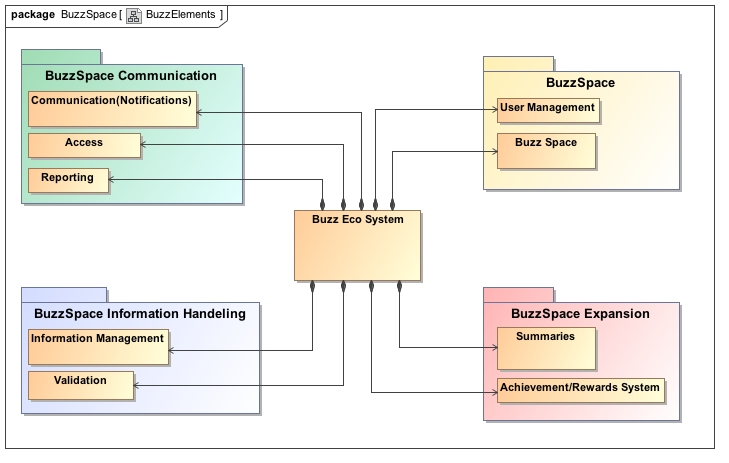
\includegraphics[width=1\textwidth] {../Hanrich/BuzzElements.jpg}\\[0.4cm]    
	\end{center}
\subsection{Introduction}
We use this document to give a high level overview of the buzz  discussion board. We have identified the various components of our system. The purpose of this document is to create a dynamic and scalable solution. We also want to include an achievement system that rewards users for using the discussion board. This document will inform you on how we will achieve a system that is both scalable and pluggable. We have identified the use cases of the various components of the discussion board and helped expand on them.
\newpage
\subsection{Use case prioritiation}
\textbf{Critical} 
\begin{itemize}
  \item BuzzSpace
  \item CRUD posts(Creating,Reading; Updating; Deleting).
  \item System Access
  \item Information Management
  \end{itemize}
\textbf{Important} 
\begin{itemize}
  \item User Management
  \item Communication(Notifications)
  \item Reporting
\end{itemize}
\textbf{Nice-To-Have} 
\begin{itemize}
  \item Achievement/Rewards System
  \item Reporting
  \item Summaries
\end{itemize}
\subsection{Use case/Service contracts}
\begin{center}
  \begin{tabular}{| p{3cm} | p{4cm} | p{4cm} | p{4cm} |}
    \hline
    Use Case & Pre Condition & Post Condition & Description \\ \hline \hline
    BuzzSpace & There must be a valid user & User must still exist & This use case provides an interface that facilitates management of threads\\ \hline
    Information Management &  &  &\\ \hline
    Communication& A user needs to be registered in order to have notifications sent to his profile inside the application. For e-mails to be sent, a valid and up-to-date e-mail address is needed on the user database. & A notification should visibally be highlighted in the application with appropriate messages. In some cases, an email is sent out from the system. & This use case specifies all the functions that the Buzz system needs to have in order to communicate important information with the user. \\ \hline
    Summaries &  &  & \\ \hline
    Achievement Rewards System & A user's level requires Achievements to be allocated and/or rewards to be awarded & Achievements are allocated and/or rewards are awarded & This use case provides a system that allocates achievements to users based on their levels and the votes they aquired. it also provides a system that awards rewards to users based on their achievements.\\ \hline
    Access & The user will need a browser to view the website. & Threads and posts are displayed in descending order by date. & Details how an end-user will be able to access the Buzz system. \\ \hline
    Validation & Post is palgiarised and/or does not follow netiquette & Post is valid against rules  & \\ \hline
    User Management & If the User is not inlvolved in the course (not a registered student/ tutor/ teaching assistant).  & The User is still involved in the course & This is a basic system which manages the User's Login and logout. \\ \hline
    Reporting & Data must be available to report on. & Data must not be corrupt. & This use case generate report for all actors\\ \hline
    \hline
  \end{tabular}
\end{center}
\subsection{Required functionality}
\begin{itemize}
\newpage
	% We need to add the correct pictures here. We must also give a description of the elements.
	\item \textbf{BuzzSpace}. A Buzz Space is a integral component of the Buzz System which facilitates the management of threads added by its users. Buzz Spaces may be created for each active module in the Computer Science Department in order to promote intuitive communication between the Computer Science staff and its students.	
		\begin{center}
  	 	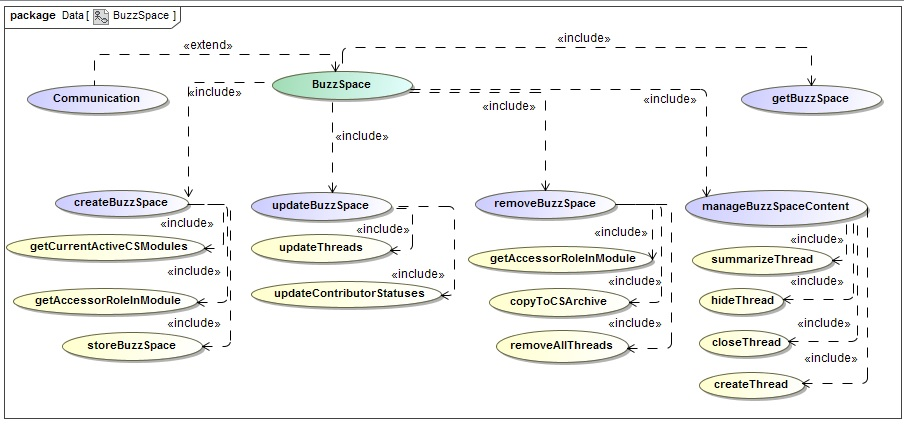
\includegraphics[width=1\textwidth] {../Lelethu/UseCase_BuzzSpace.jpg}\\[0.4cm]    
		\end{center}
\newpage
\item \textbf{Validation}. This module will be used to make sure that post follow certain rules and help generate certain reports regarding these rules.
		\begin{center}
  	 	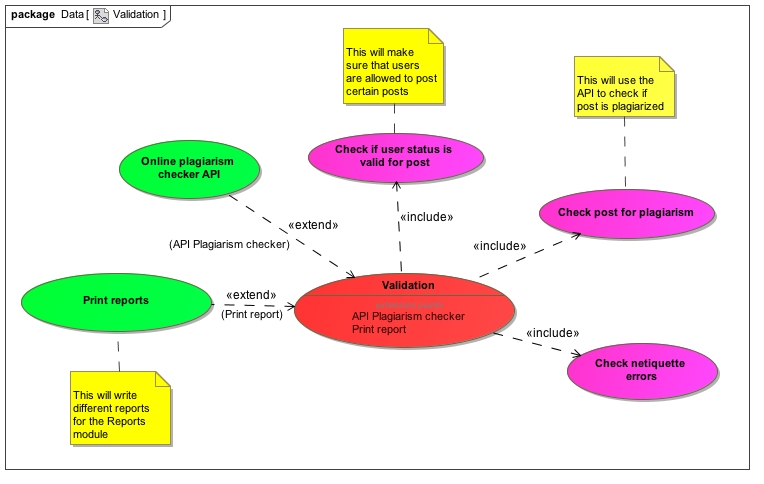
\includegraphics[width=1\textwidth] {../Chris/Validation.jpg}\\[0.4cm]    
		\end{center}
\item  \textbf{Information Management}
		\begin{center}
  	 	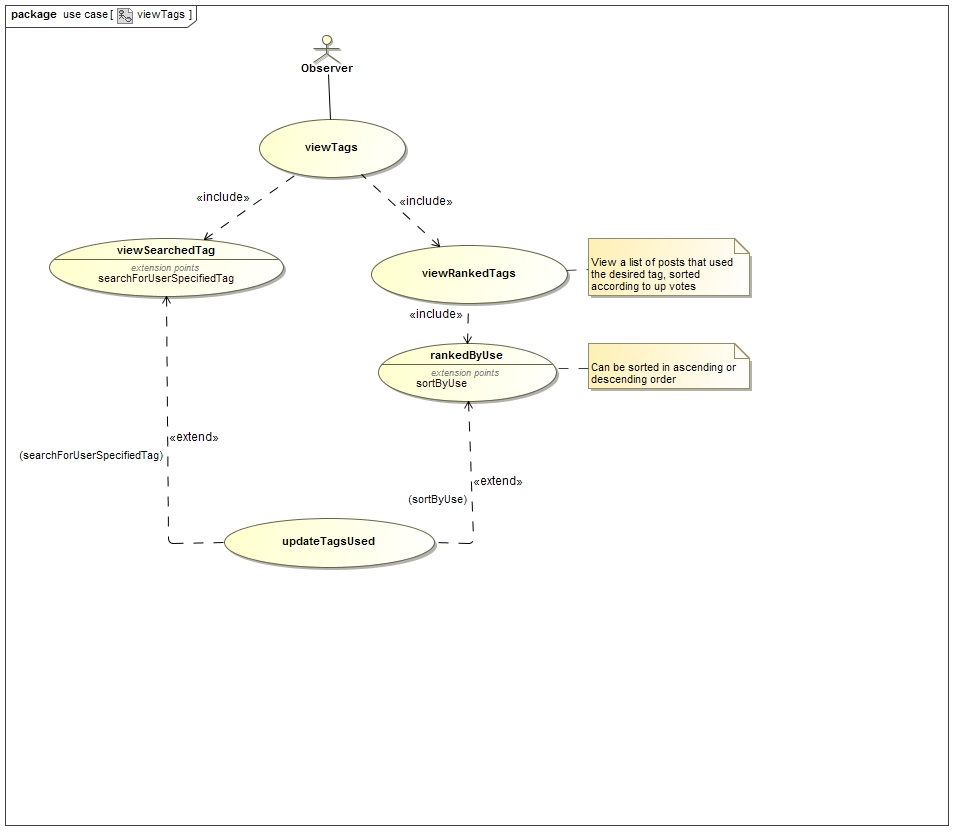
\includegraphics[width=1\textwidth] {../Herman/viewTags.jpg}\\[0.4cm]    
		\end{center}
\item \textbf{Reporting}. We will use the reporting module to generate quite a few reports regarding the Buzz Space system. It will be a key player in adding value to lecturers and students. Each student can easily general a report regarding their own contributions towards a Buzz Space. Lecturers will be able to grade student performance and see how much plagiarism has occurred. The system administrators will be able to check for system bugs and see error logs. 
		\begin{center}
  	 	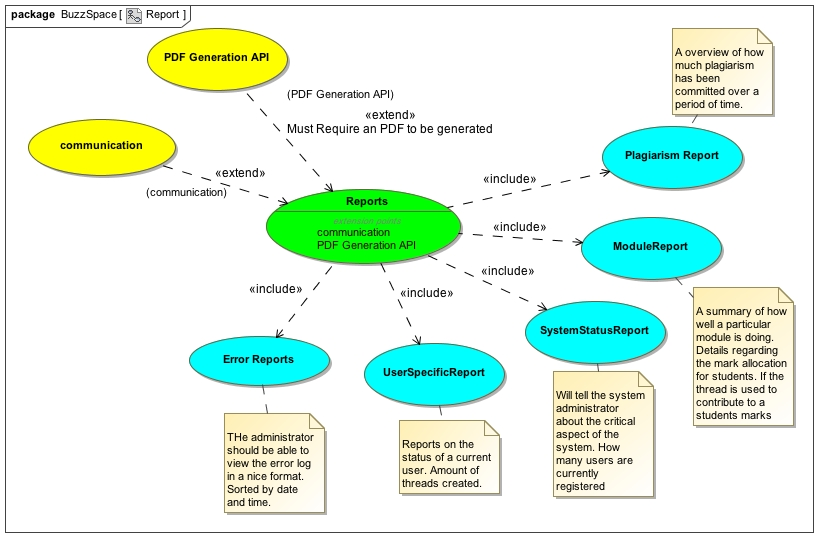
\includegraphics[width=1\textwidth] {../Hanrich/Report.jpg}\\[0.4cm]    
		\end{center}
\newpage
	\item \textbf{Communication (Notifications)}
		\begin{flushleft}
		This module describes the way the Buzz System will communicate with its users inside of the application as well as sending information and/or reports from the Buzz system to an external system such as email notifications.
		\end{flushleft}
		\begin{center}
		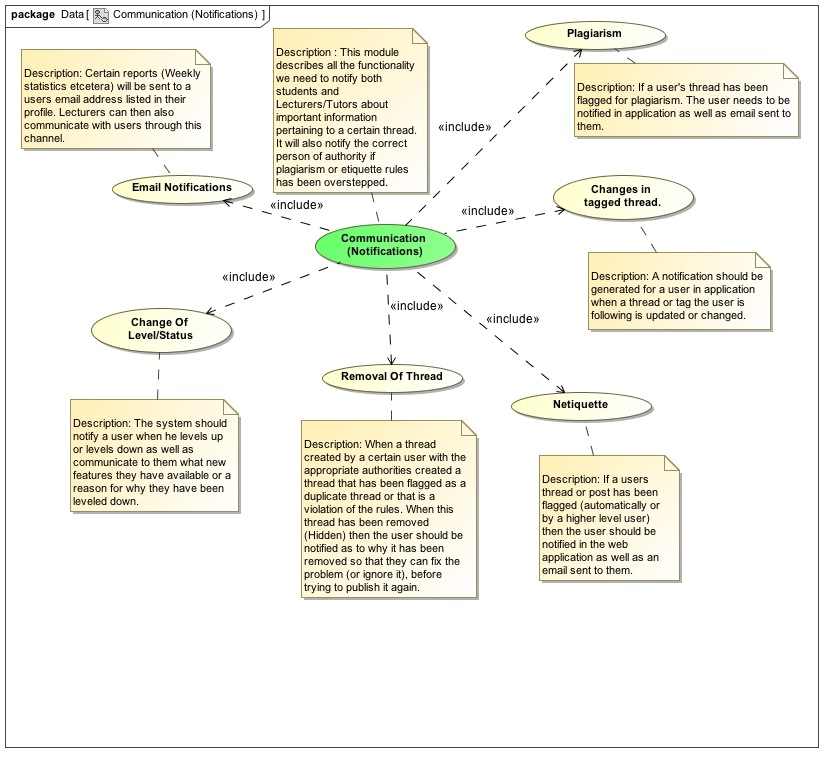
\includegraphics[width=1\textwidth]{../Jason/Communication_(Notifications).jpg}\\[0.4cm]
		\end{center}
	\item \textbf{Access}
		\begin{flushleft}
		The use case below shows how a end-user will be able to access the Buzz system. Although a user may not be registered, they should still be able to view and read threads and posts.
		\end{flushleft}
		\begin{center}
		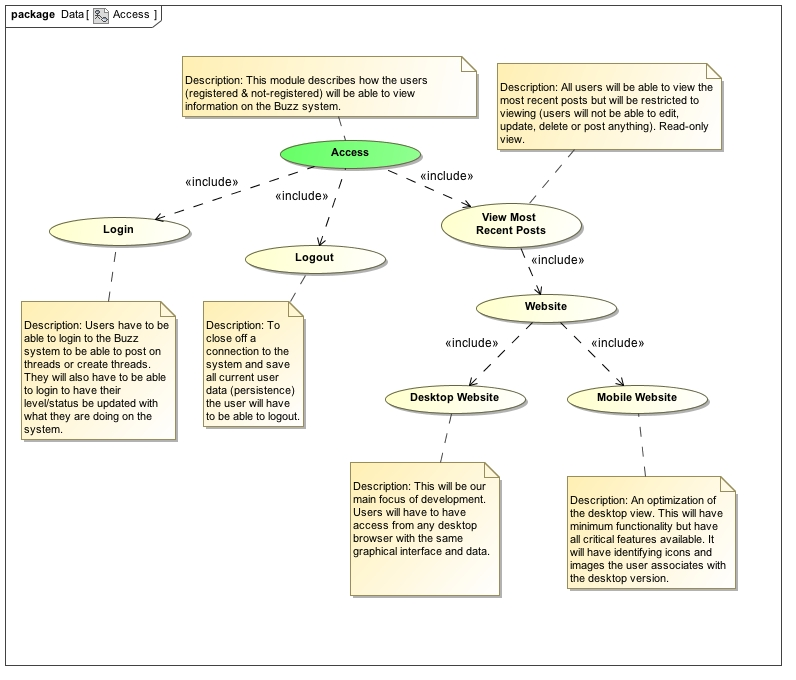
\includegraphics[width=1\textwidth]{../Jason/Access.jpg}\\[0.4cm]
		\end{center}
\item \textbf{User Management}
		\begin{flushleft}
		This use case specifies how the user's themselves will be managed (not their data). This refers to who will be allowed to firstly login, access a buzzspace and then a specific thread and eventually logout. This displays what services help acheive User Management and also which servies are subsets of other services.
		\end{flushleft}
		\begin{center}
		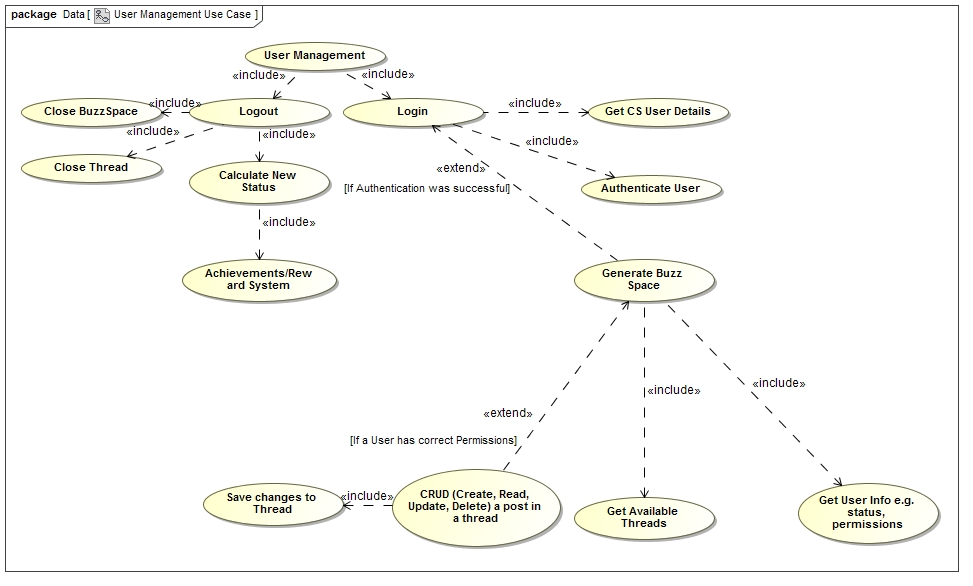
\includegraphics[width=1\textwidth]{../Kale-ab/UserManagementUseCase.jpg}\\[0.4cm]
		\end{center}
	\item \textbf{Achievement/Rewards system}
		\begin{flushleft}
		The Achievement/Rewards system use case component shows how the Buzz System generates and awards rewards to users, based on their different achievements. The achievemnet is derived from each user's level of participation on the Buzz Space as well as the number of votes they acquire. The Achievement/Reward system incorporates the gamification functionality of the Buzz System. Therefore, forcing the users of the system to participate more often as there will be rewards for this.
		\end{flushleft} 
		\begin{center}
		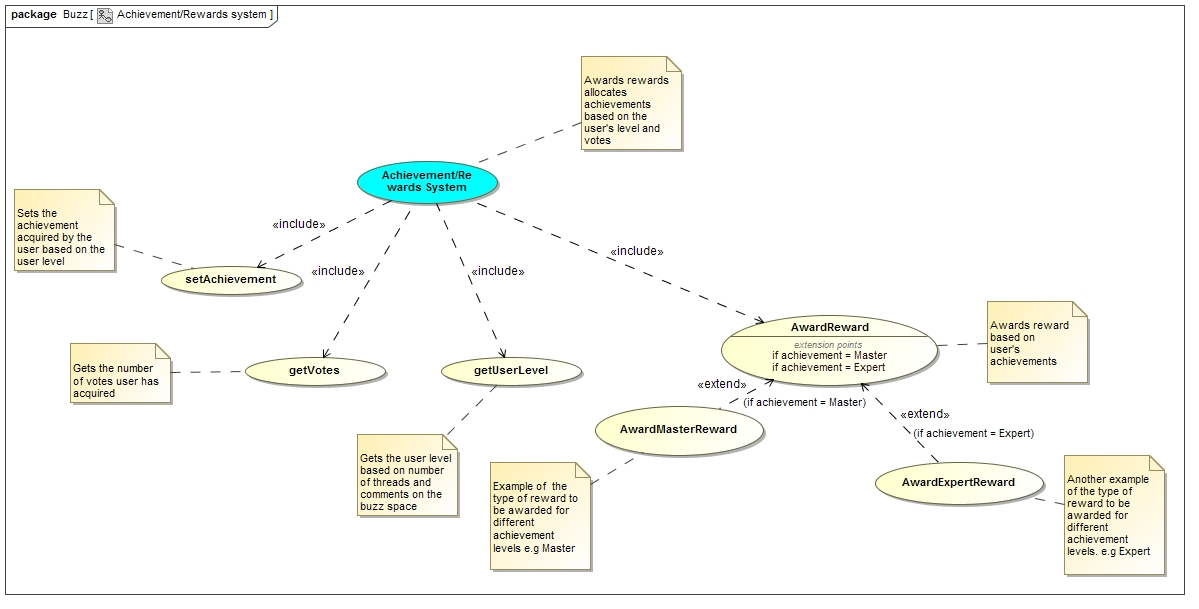
\includegraphics[width=1\textwidth]{../Goodness/Achievement_Rewards_System_Use_case_Diagram.jpg}\\[0.4cm]
		\end{center}
\end{itemize}
\subsection{Process specification}
We want to show various important process specification of our recommendation.
\begin{itemize}
	\item CreateBuzzSpace
		\begin{center}
  	 	\includegraphics[width=1\textwidth] {../Functional_Requirements_Diagrams/ActivityDiagrams/ActivityDIagram_CreateBuzzSpace.jpg}\\[0.4cm]    
		\end{center}
	\item Validation
		\begin{center}
  	 	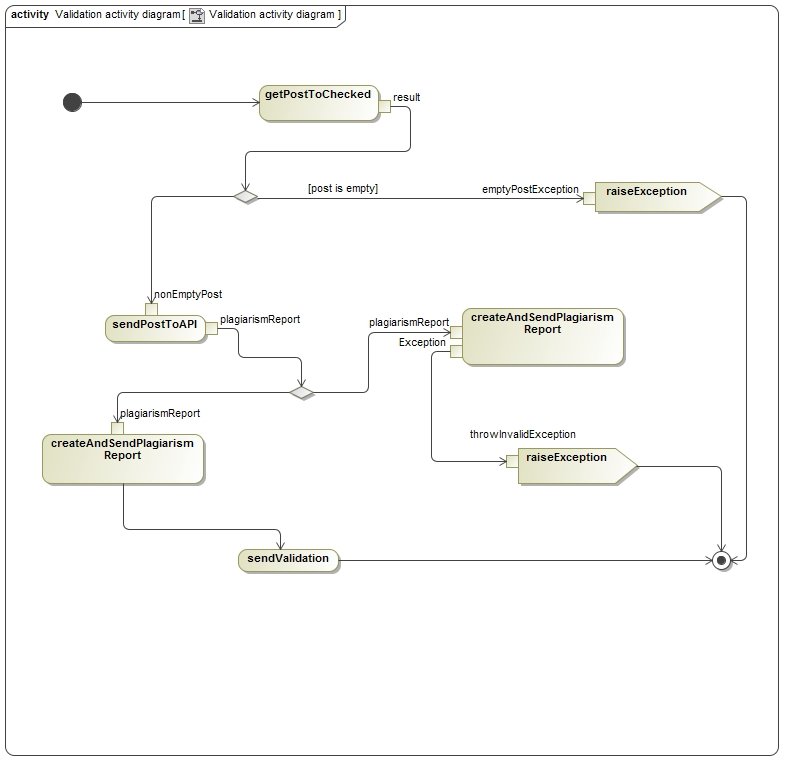
\includegraphics[width=1\textwidth] {../Chris/Validationactivitydiagram.jpg}\\[0.4cm]    
		\end{center}
	\item Achievement/Rewards system
		\begin{center}
		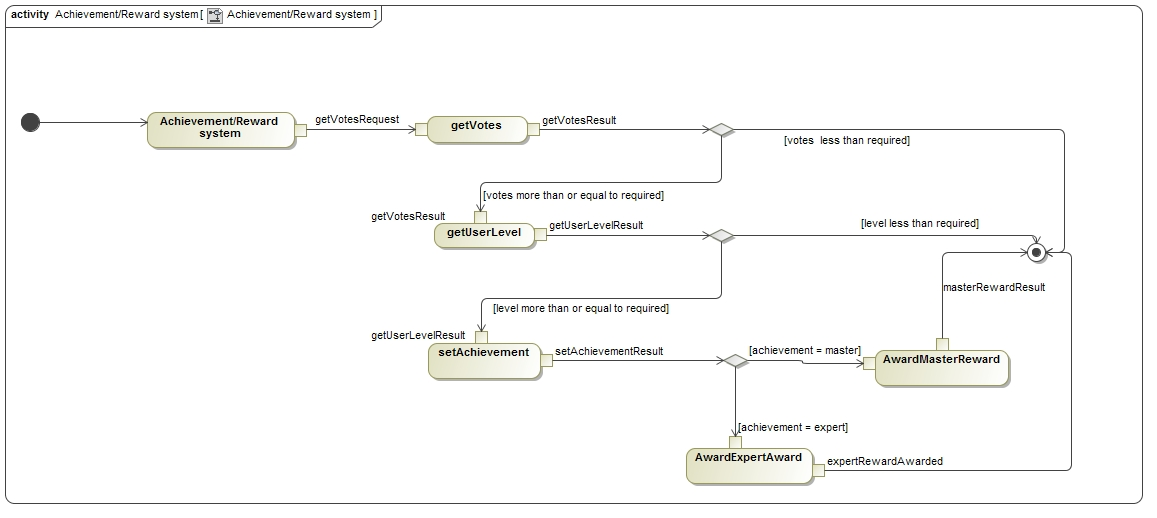
\includegraphics[width=1\textwidth]
		 {../Goodness/Achievement_Rewards_System_ActivityDiagram.jpg}\\[0.4cm]
		\end{center}
\end{itemize}
\subsection{Domain Model}
	\begin{center}
  	 	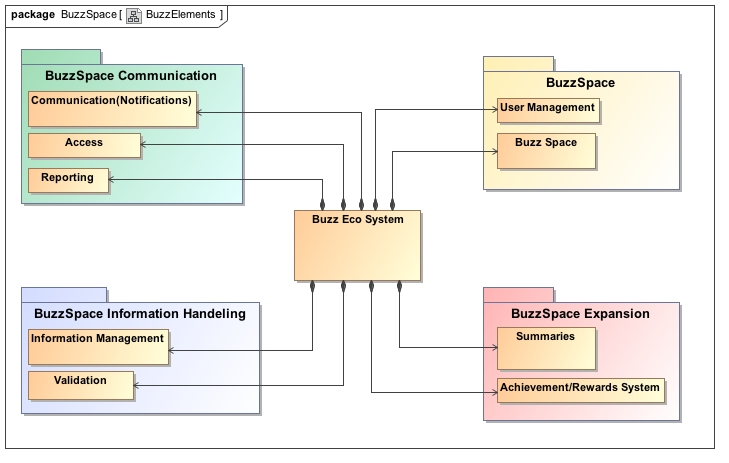
\includegraphics[width=1\textwidth] {../Hanrich/BuzzElements.jpg}\\[0.4cm]    
	\end{center}
\index{Vision}
\newpage


\bibliography{myrefs}{} 
\bibliographystyle{ieeetr}
\end{document}
